% What follows the % sign is interpreted by latex as a comment

% The following two lines declare the type of document, the size of the
% font and the fact that we will use the epsfig file in the package dvips

\documentclass[12pt,dvips]{article}
\usepackage[dvips]{epsfig}

% These two lines set the indent and extra line spacing at the beginning 
% of a paragraph (they may be omitted, which will produce default values)

\parindent 0pt
\parskip 1mm

\begin{document}

% The document environment allows one to make a title, sections with
% headings etc.  Here we will just use boldface (\bf), \Large and \large 
% to increase the font size, and the center environment to produce titles 
% and headings.

\begin{center}
{\Large\bf PY 421 - Introduction to Computational Physics}

% remember to close all { with a matching }

% \bigskip \medskip and \smallskip produce various amounts of vertical space
\bigskip     

{\large\bf Homework \# 3}
\smallskip
% remember to leave an empty line between paragraphs, otherwise latex
% will merge the lines

{\large\bf Your Name}
\end{center}

\bigskip
{\bf Answer to problem 2}
\bigskip

We use the epsfig command to insert Figure~\ref{pict1} in the text.
% (the ~ sign is used to make sure that Figure is not separated
% from the number by a line break)
Change the name of the figure in the epsfig command from
sample\_fig1.eps to the name of the figure you want to display.
Notice the use of label and of ref.  Any name can be used as
a label, but each label must be associated with a unique name. 
The center environment is used to place the figure in the center
of the page.
[h!] is used to force the placement of the figure here.  Latex
has a mind of its own about figure placement.  Other options are
[t] for top, [b] for bottom.  Try.

\begin{figure}[h!]
\begin{center}
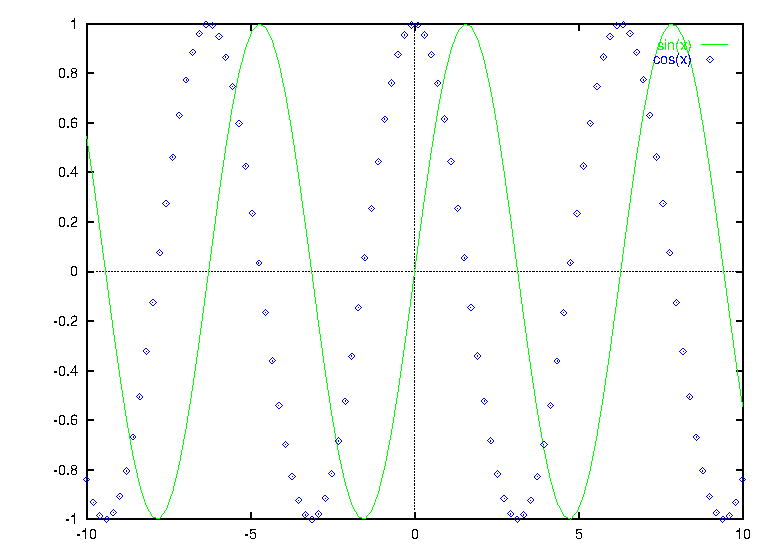
\epsfig{file=sample_fig1,width=11cm,height=8cm}
\end{center}
\caption{\label{pict1}This is the first graph in my report.}
\end{figure}

% The following forces a new page
\vfil\eject
{\bf Answer to problem 3}
\bigskip

Mathematical expressions can be incorporated in the text by enclosing
them with \$ signs.  Remember to close all \$ with a matching \$.
Here are a few mathematical expressions: $a=b+c+\cos(\phi)$,
$\alpha=\beta+\gamma+\Phi-\Lambda$ (notice the way Greek letters
are entered).  $N=m \times l$.  $q=\sqrt{f+2 c}$.  See how to 
introduce upper and lower indices: $r^2=x^2+y^2, r=\sqrt{x^2+y^2},
a_i^n=2 b_j^\phi$.  Notice the use of the brackets for composite
indices: $v_i=\sum_j a_{i,j} w_j$, $x=e^{\log(x)}$.
In the following, we introduce some extra space:
$a a \, a \; a \quad a \qquad a$.  The following symbols are
useful: $ <, \le, \ll, >, \ge, \gg, \sim, \approx, \infty, \ne$.

Standalone mathematical equations (not in the text) can be
typeset by enclosing them in the equation environment:
\begin{equation}
A = \int_0^\infty e^{-x^2} dx
\label{gauss}
\end{equation}
Labels are not mandatory, but they allow us to make reference
to Eq.~\ref{gauss}.

Notice the use of fractions:
\begin{equation}
\rho=\frac{1}{2} \frac{1+x^2}{a+\sqrt{y+3}} \frac{1+\cos^2(x)}{\log(y)+2} 
\label{fraction}
\end{equation}
(I am not sure that Eq.~\ref{fraction} makes much sense.)
Notice also how to make parenthesis bigger
\begin{equation}
f(x)=\big( \sin(x) \big) \Big[ \frac{e^x+1}{e^{-x}+1} \Big]
\Bigg( \frac{\int_0^x \frac{\sin(x')}{x'}dx'}{x^2+1} \Bigg) 
\label{big}
\end{equation}

Multiline equations can be composed with the eqnarray environment:
\begin{eqnarray}
a=x+y+z \\
+ \rho^2
\label{array1}
\end{eqnarray}
Notice the use of nonumber
\begin{eqnarray}
a=x+y+z \nonumber \\
+ \rho^2
\label{array2}
\end{eqnarray}
Finally, in a multiline equation, it is possible to align
the expressions as follows:
\begin{eqnarray}
f_1(x)&=&x+\exp[\sin(x)]  \\
g_1(x)+f_2(x)&=& x^2-1  \\
y &=& \int f_2(x) dx 
\label{multiline}
\end{eqnarray}

\bigskip
{\bf Answer to problem 4}
\bigskip

Our final results are reproduced in Fig.~\ref{pict2}. 
\begin{figure}[h!]
\begin{center}
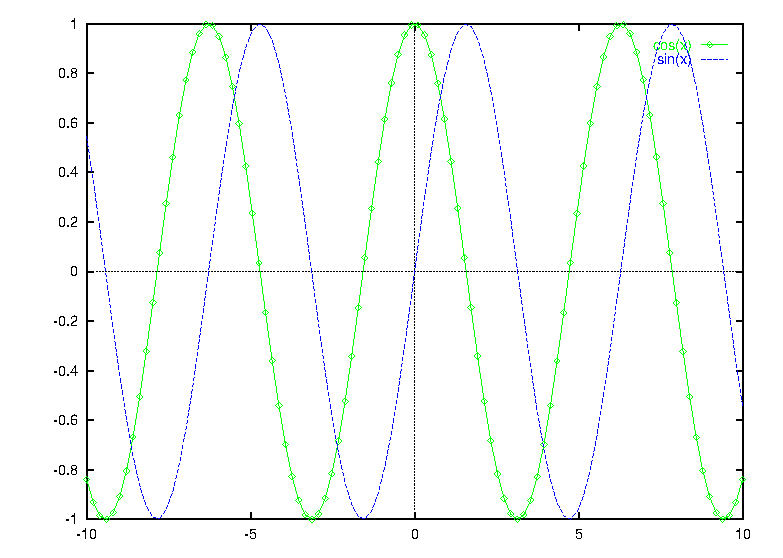
\epsfig{file=sample_fig2,width=11cm,height=8cm}
\end{center}
\caption{\label{pict2}This is the second graph in my report.}
\end{figure}

Remember to end the document environment.

\end{document}
